\section{Kartoteket - Daniel Rapp}
\subsection{Inledning}
Idag är information om Region Östergötlands operationsartiklar, så som priserna och
placeringen i lagret på tandborstar, tandkräm, handskar och annan
medicinsk utrustning, hanterat av ett internt system.
Detta system kallas ett "\textit{kartotek}", och är helt enkelt en sorts artikeldatabas.
I vårt system så ska detta uppdateras och förbättras på olika sätt.

\subsubsection{Syfte}
Syftet med denna del är att beskriva vad kartoteket är samt
hur vår förbättrade lösning är uppbyggd.


\subsubsection{Frågeställning}
Frågeställningar:
\begin{itemize}
  %\item Kan man implementera ett kartotekssystem som uppfyller kundens önskemål?
  %\item Går det att implementera ett kartotekssystem som 
  \item Går det att integrera systemet för handböcker med kartoteket utan att förlora funktionalitet?
\end{itemize}


\subsubsection{Avgränsningar}
%Förutom ett förbättrat kartotekssystem så är Region Östergötland också i behov av
%ett bättre system för att hantera deras lager på ett mer automatiserat sätt.
%Bland annat så skulle de behöva ett system som låter dem checka in vilka varor från lagret de hämtat
%ut, istället för att checka av manuellt, vilket kan vara felbenäget.

%Vi valde dock att avgränsa oss från att bygga denna lösning, på grund av tidsbrister.
%Istället fokuserade vi på att förbättra kärnfunktionaliteten i applikationen.

\clearpage
\subsection{Bakgrund}
I dagsläget använder Region Östergötland sig av två separata system
för att förbereda operationer. En handbok (se ovan) och ett kartotek (se \ref{fig:kartotek}).
Dessa är för tillfället helt separata applikationer.

\begin{center}
  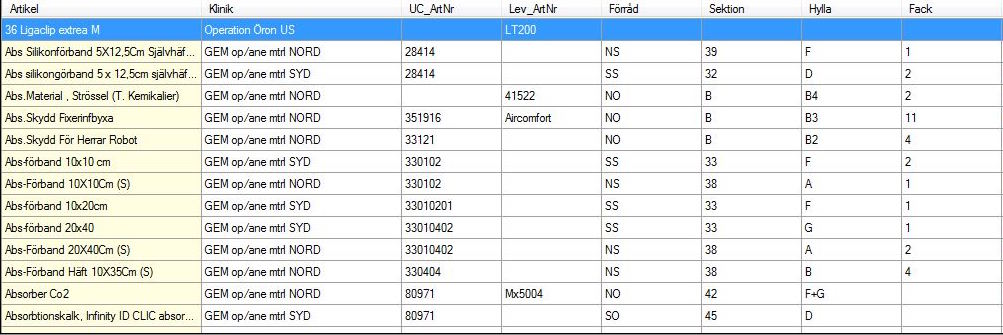
\includegraphics[width=0.9\textwidth]{../images/forradsinfo.jpg}
  \label{fig:kartotek}
\end{center}

Så om en artikel slutas säljas eller Region Östergötland
väljer att inte köpa in en viss artikel längre så tar de bort artikeln
från kartoteket. Problemet som då uppstår är att detta inte reflekteras
i handböckerna. Så om t.ex. en "\textit{Oral-B Pro 600 CrossAction}"\ tandborste används i
en "\textit{Laparoskopisk sigmoideumresektion}", och tandborsten slutas säljas
så tas den bort från kartoteket, men eftersom handboken för operationen inte är
kopplad till kartoteket så uppdateras det inte att denna artikel inte längre finns i lagret.

Vår förbättrade lösning
integrerar systemet som hanterar handböcker tillsammans med ett nytt kartotek,
där allesammans är byggt på webben. När en artikel ändras eller tas bort i kartoteket
så ändras den även i alla handböcker för operationer som kräver denna artikel.



%\subsection{Teori}
\subsection{Metod}
Precis som resten av systemet så är kartoteket skrivet på webben, och
därmed i javascript, html och css.

TODO: Skriv mer.

\clearpage
\subsection{Resultat}
Resultatet av vårt arbete är ett förbättrat kartotekssystem
som integrerar data från handboken till ett
uniformt system.

Kärnfunktionaliteten i kartoteket är möjligheten att se, modifiera och hitta artiklar.
Så denna del är uppdelad i tre delar.

\subsubsection{Att se artiklarna}
När man först kommer in på sidan för att hantera kartoteket så
blir man välkomnad av en stor tabell som innehåller alla artiklar
i kartoteket (runt 3000 för tillfället). Se figur \ref{fig:table}
\begin{center}
  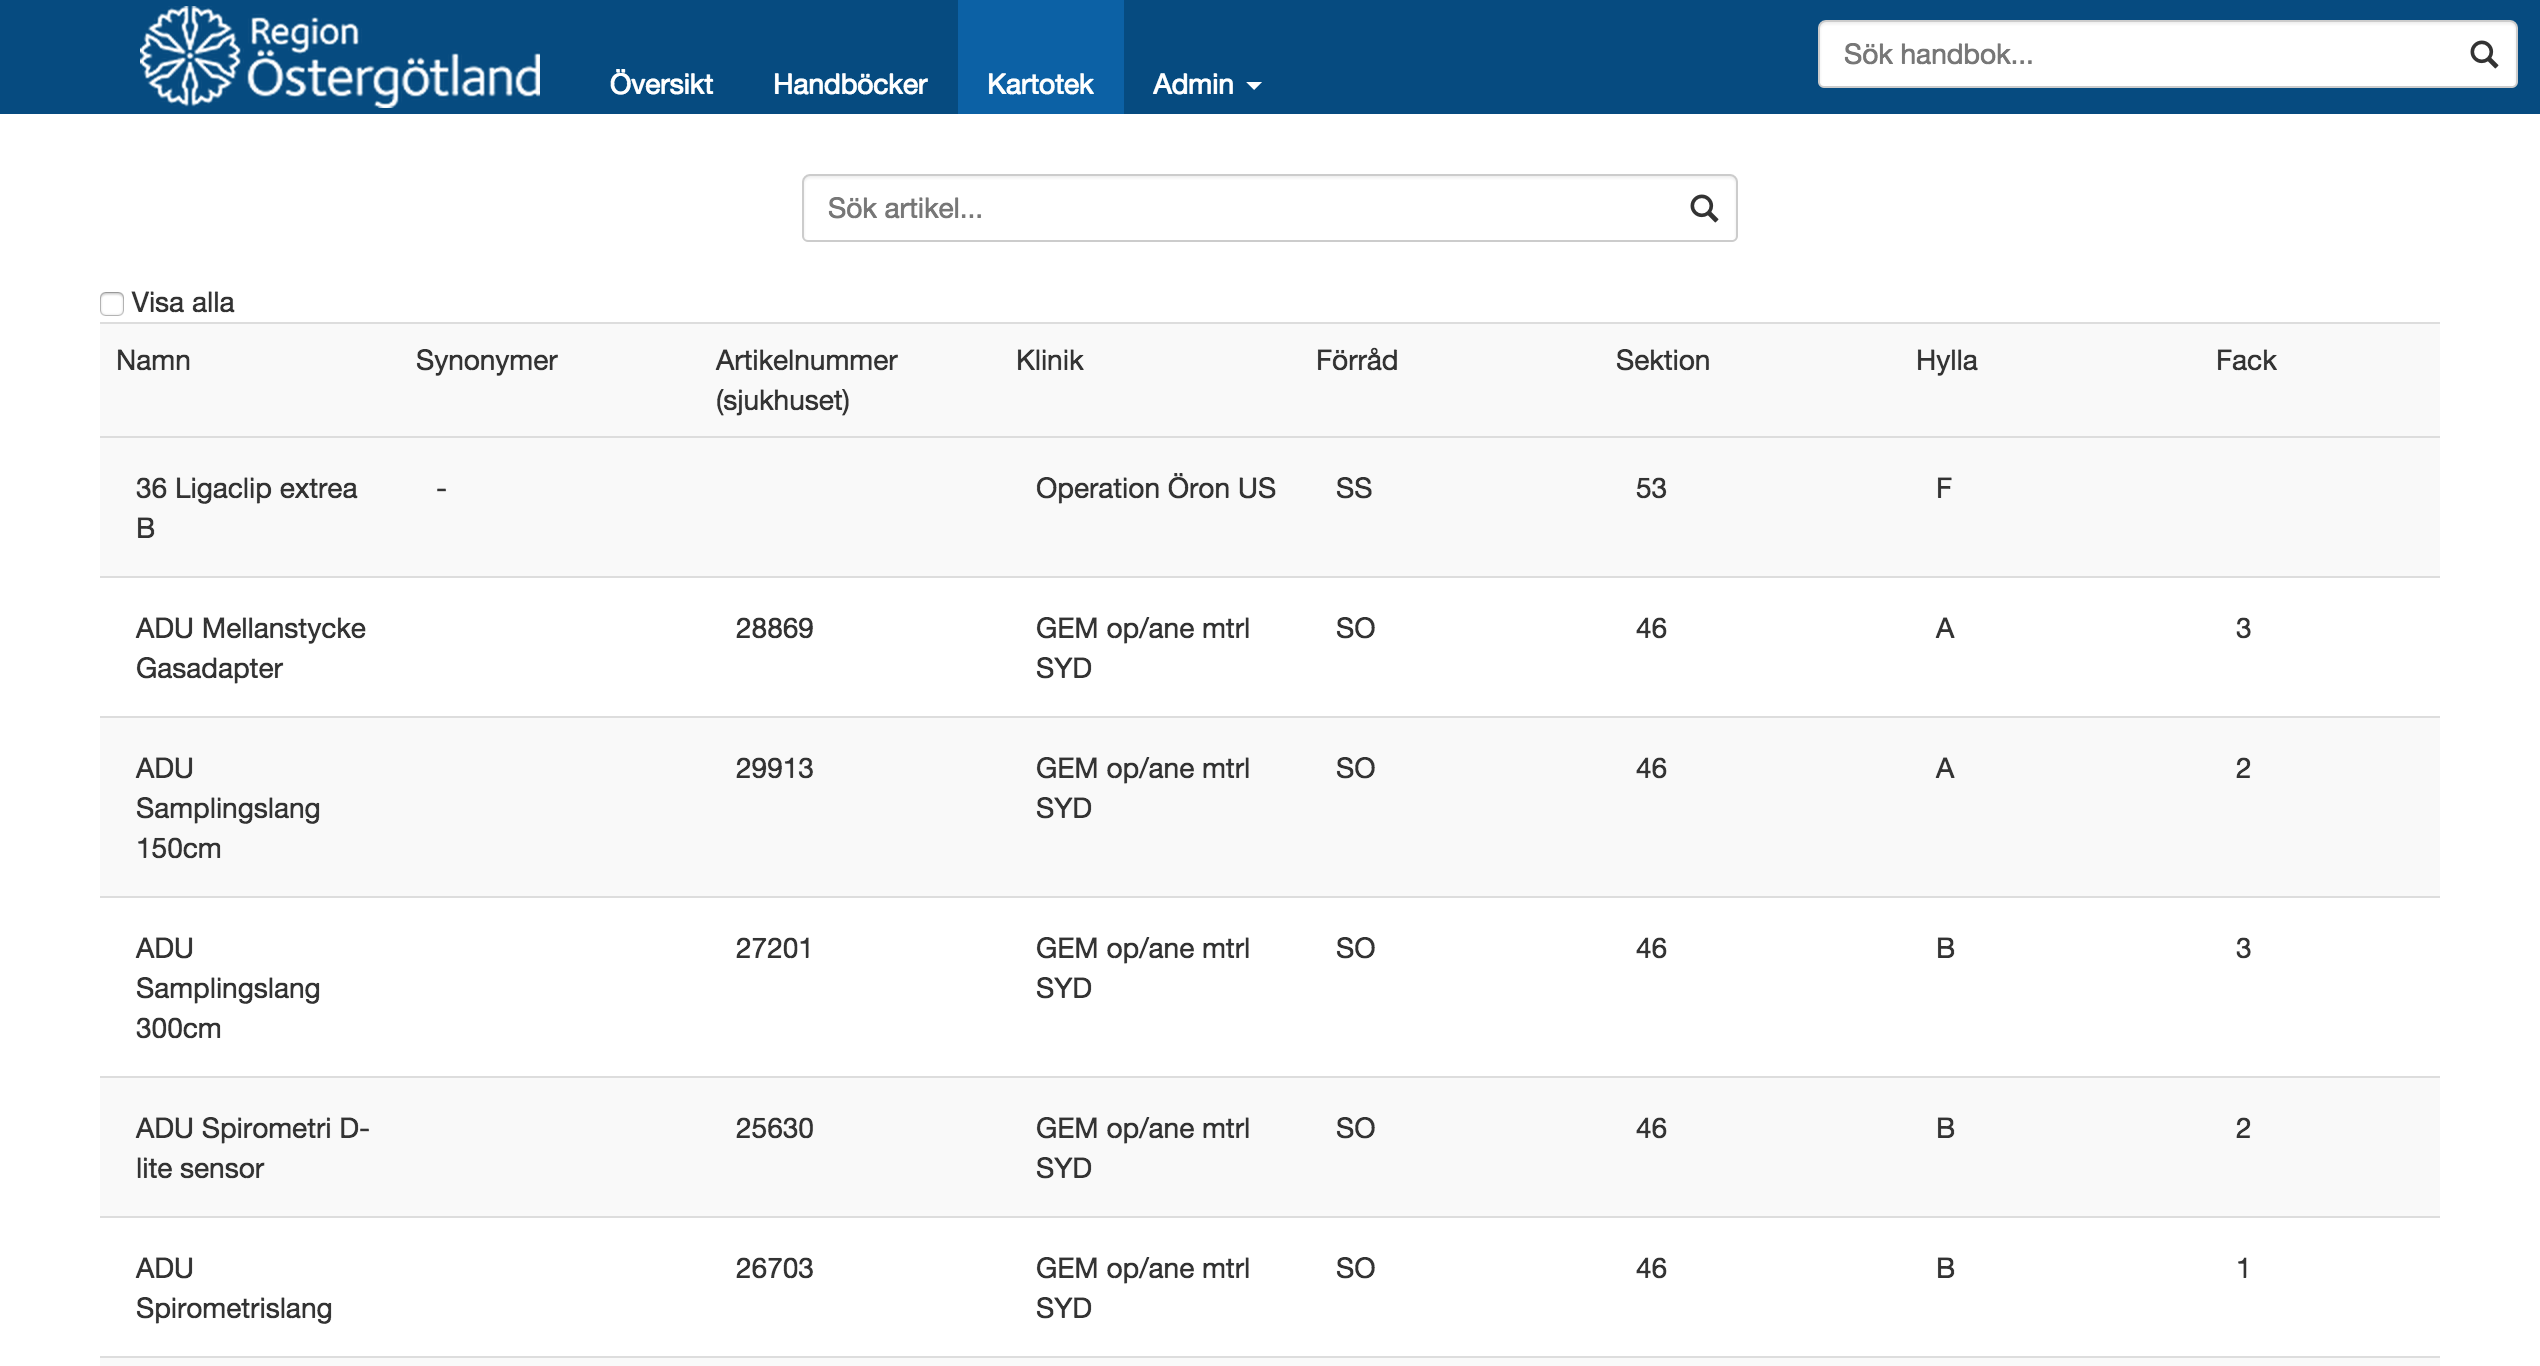
\includegraphics[width=0.9\textwidth]{../images/kartotek1.png}
  \label{fig:table}
\end{center}
När man först kommer in så laddas endast runt 50 artiklar, men
om man skrollar ner så laddas fler.

Det finns två olika sätt att se informationen.
Två olika vyer.

Den ena är standardvyen, som man ser om man inte är inloggad
eller inte är administratör. Denna vyn kan ses i \ref{fig:table}
och innehåller endast den mest nödvändiga informationen om
artiklarna, som namn, klinik, förråd, etc.

Den andra vyn är administratörsvyn.
Man kommer endast in på denna vy om man är administratör.
Om man aktiverar denna så utvidgas tabellen för att
visa mer information om artiklarna, bland annat pris på artiklarna.
Vi har valt att inte inkludera en bild på denna information
då detta är sekretessbelagt.

I den här vyn finns också möjligheten att ta bort, lägga och modifiera
information om artiklar, vilket är vad nästa två delarna handlar om.

\clearpage
\subsubsection{Modifiering av artiklarna}


\subsubsection{Sökning av artiklarna}



\subsection{Diskussion}
Har vi lyckats med kartoteket? Och framför allt, är
kunden nöjd? Fick kunden de dom önskade?

\subsubsection{Resultat}


\subsubsection{Metod}


\subsection{Slutsatser}
%Allt som allt så blev vi väldigt nöjda med kartoteket.


\subsection{Referenser}
\vspace{-9mm}
\renewcommand{\refname}{}
\begin{thebibliography}{9}

\end{thebibliography}
